% Created 2021-09-11 Sat 08:17
% Intended LaTeX compiler: xelatex
\documentclass[letterpaper]{article}
\usepackage{graphicx}
\usepackage{grffile}
\usepackage{longtable}
\usepackage{wrapfig}
\usepackage{rotating}
\usepackage[normalem]{ulem}
\usepackage{amsmath}
\usepackage{textcomp}
\usepackage{amssymb}
\usepackage{capt-of}
\usepackage{hyperref}
\usepackage[margin=1in]{geometry}
\usepackage{fontspec}
\usepackage{indentfirst}
\setmainfont[ItalicFont = LiberationSans-Italic, BoldFont = LiberationSans-Bold, BoldItalicFont = LiberationSans-BoldItalic]{LiberationSans}
\newfontfamily\NHLight[ItalicFont = LiberationSansNarrow-Italic, BoldFont       = LiberationSansNarrow-Bold, BoldItalicFont = LiberationSansNarrow-BoldItalic]{LiberationSansNarrow}
\newcommand\textrmlf[1]{{\NHLight#1}}
\newcommand\textitlf[1]{{\NHLight\itshape#1}}
\let\textbflf\textrm
\newcommand\textulf[1]{{\NHLight\bfseries#1}}
\newcommand\textuitlf[1]{{\NHLight\bfseries\itshape#1}}
\usepackage{fancyhdr}
\pagestyle{fancy}
\usepackage{titlesec}
\usepackage{titling}
\makeatletter
\lhead{\textbf{\@title}}
\makeatother
\rhead{\textrmlf{Compiled} \today}
\lfoot{\theauthor\ \textbullet \ \textbf{2021-2022}}
\cfoot{}
\rfoot{\textrmlf{Page} \thepage}
\titleformat{\section} {\Large} {\textrmlf{\thesection} {|}} {0.3em} {\textbf}
\titleformat{\subsection} {\large} {\textrmlf{\thesubsection} {|}} {0.2em} {\textbf}
\titleformat{\subsubsection} {\large} {\textrmlf{\thesubsubsection} {|}} {0.1em} {\textbf}
\setlength{\parskip}{0.45em}
\renewcommand\maketitle{}
\author{Houjun Liu}
\date{\today}
\title{Resistivity and Conductivity}
\hypersetup{
 pdfauthor={Houjun Liu},
 pdftitle={Resistivity and Conductivity},
 pdfkeywords={},
 pdfsubject={},
 pdfcreator={Emacs 27.2 (Org mode 9.4.4)}, 
 pdflang={English}}
\begin{document}

\maketitle


\section{Resistance}
\label{sec:org930ca11}
So, let's figure out resistance.

We know that\ldots{} \(V\) = \(\frac{J}{C}\), per
\href{KBhPHYS201Voltage.org}{KBhPHYS201Voltage}, and we also know that
resistance would equal a unit \(\frac{Vs}{c}\) given that
\(I = \frac{C}{s} = \frac{\Delta V}{Resistance}\) (see
\href{KBhPHYS201Current.org}{KBhPHYS201Current} Current). Plugging in
the definition of voltage, we get that resistance is measured in
\(\frac{Js}{C^2}\). We call this unit Ohms, or \(\Omega\).

\definition{Resistance $\Omega$}\{A value measured in \(\frac{Js}{C^2}\) that measures the resistance to current\}
\subsubsection{Calculating resistance}
\label{sec:org289a47c}
\begin{itemize}
\item So, let's think. With a wire of length L and with a wire of area A, if
we increase L, the resistance in the wire would increase; if we
increase area A, the resistance in the the wire would decrease.
\item \(Resistance = \frac{L}{A}*ResistivityOfMaterial\) with units
\(\frac{m}{m^2}(\Omega \times m)\).
\end{itemize}

Sometimes its easier to think about conductivity.

and, indeed, resistivity of materials are measured in
\(\Omega \times m\), which also makes sense intuitively.

\subsubsection{Heat of resistance}
\label{sec:org1b5e0d5}
\begin{figure}[htbp]
\centering
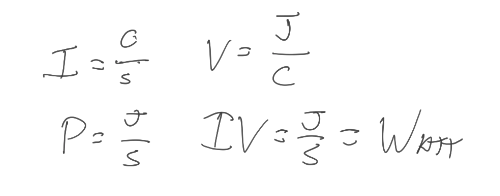
\includegraphics[width=.9\linewidth]{KBe20phys250srcHeatFromResistors.png}
\caption{KBe20phys250srcHeatFromResistors.png}
\end{figure}

\section{Ohm}
\label{sec:orgfb5d86a}
\[\Omega = \dfrac{\text{V}}{\text{A}} = \dfrac{1}{\text{S}} = \dfrac{\text{W}}{\text{A}^2} = \dfrac{\text{V}^2}{\text{W}} = \dfrac{\text{s}}{\text{F}} = \dfrac{\text{H}}{\text{s}} = \dfrac{\text{J} {\cdot} \text{s}}{\text{C}^2} = \dfrac{\text{kg} {\cdot} \text{m}^2}{\text{s} {\cdot} \text{C}^2} = \dfrac{\text{J}}{\text{s} {\cdot} \text{A}^2}=\dfrac{\text{kg}{\cdot}\text{m}^2}{\text{s}^3 {\cdot} \text{A}^2}\]
(Wikipedia)
\end{document}
